\begin{pastexam}[label={px:ntu-109-dsaa-14}]{臺大資工所 109 學年度 第 14 題}
（問答）

(20 points) A tree $T$ is assumed to be simple, undirected, and with \textbf{positive
edge-weights}. Let $d_T(u,v)$ denote the distance between $u$ and $v$ on $T$. For a vertex $v$,
the \textit{eccentricity} of $v$ is the maximum of the distance to any vertex in the tree, i.e.,
$\max_{u\in V}\{d_T(v,u)\}$. The \textit{diameter} of a tree is the maximum of the eccentricity
of any vertex in the tree. (The term ``diameter'' is overloaded. It is defined as the maximum
eccentricity and also as the path of length equal to the maximum eccentricity.) The
\textit{radius} of a tree is the minimum eccentricity among all vertices in the tree, and a
\textit{center} of a tree is a vertex with eccentricity equal to the radius.
\begin{enumerate}[label=(\alph*)]
\item (5 points) Prove or disprove that there exists a tree with three different diameters and
two centers.
\item (5 points) Prove or disprove that there exists a tree with three centers.
\item (10 points) Prove or disprove that any center of a given tree $T$ must lie in the diameter
of $T$.
\end{enumerate}
\end{pastexam}

\begin{pastsoln}
答案：(a) 存在（成立）；(b) 不存在（不成立），樹最多兩個中心；(c) 成立，而且每一個中心都在\textbf{每一條}
直徑路徑上。

記號：$d(u, v)$ 就是 $d_T(u, v)$，$\mathrm{ecc}(v)$ 是 $v$ 的離心率，$D$ 是直徑的長度。 (a) 的「three
different diameters」照題目括號裡的說明，指三條不同的、長度等於 $D$ 的路徑。

\textbf{(a) 成立，舉例}。 邊長都是 $1$：$c_1$、$c_2$ 相連，$c_1$ 再接一個葉節點 $a$，$c_2$ 再接三個葉節點
$b_1, b_2, b_3$。
\begin{center}
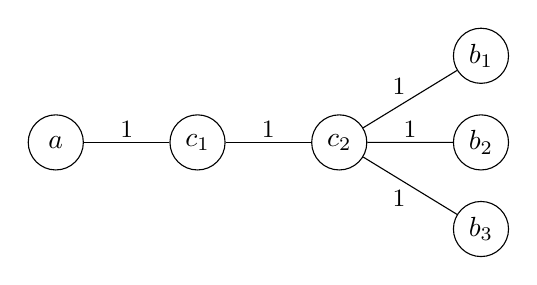
\begin{tikzpicture}[x=1cm,y=1cm,v/.style={circle,draw,inner sep=0pt,minimum size=7mm},
    w/.style={inner sep=1.5pt,font=\small}]
\node[v] (a) at (0,0) {$a$};
\node[v] (c1) at (1.8,0) {$c_1$};
\node[v] (c2) at (3.6,0) {$c_2$};
\node[v] (b1) at (5.4,1.1) {$b_1$};
\node[v] (b2) at (5.4,0) {$b_2$};
\node[v] (b3) at (5.4,-1.1) {$b_3$};
\draw (a)--node[w,above]{1}(c1) (c1)--node[w,above]{1}(c2);
\draw (c2)--node[w,above left]{1}(b1) (c2)--node[w,above]{1}(b2) (c2)--node[w,below left]{1}(b3);
\end{tikzpicture}
\end{center}
各點的離心率：
\begin{itemize}
\item $a$：到 $b_1, b_2, b_3$ 都是 $3$，$\mathrm{ecc}(a) = 3$。
\item $b_i$：到 $a$ 是 $3$，到另外兩個 $b$ 是 $2$，$\mathrm{ecc}(b_i) = 3$。
\item $c_1$：到 $a$ 是 $1$，到 $b_i$ 是 $2$，$\mathrm{ecc}(c_1) = 2$。
\item $c_2$：到 $a$ 是 $2$，到 $b_i$ 是 $1$，$\mathrm{ecc}(c_2) = 2$。
\end{itemize}
直徑 $D = 3$，距離是 $3$ 的點對只有 $\{a, b_1\}$、$\{a, b_2\}$、$\{a, b_3\}$，所以恰好有三條直徑
$a\,c_1\,c_2\,b_1$、$a\,c_1\,c_2\,b_2$、$a\,c_1\,c_2\,b_3$。 半徑是 $2$，中心是 $c_1$、$c_2$ 兩個。 這棵樹
同時有三條直徑和兩個中心，所以命題成立。

(b)(c) 都靠下面這個引理。

\textbf{引理}。 設 $P$ 是任意一條直徑，兩端是 $a$、$b$，$d(a, b) = D$。 對每個頂點 $v$，令 $w$ 是 $P$ 上
離 $v$ 最近的頂點（$v$ 在 $P$ 上時 $w = v$）。 則
\[
\mathrm{ecc}(v) = \max\bigl(d(v, a),\ d(v, b)\bigr) = d(v, w) + \max\bigl(d(w, a),\ d(w, b)\bigr).
\]

\textbf{引理的證明}。 樹上兩點之間只有一條簡單路徑。 $v$ 到 $w$ 的路徑除了 $w$ 不碰到 $P$（否則有更近的點），
接上 $P$ 從 $w$ 到 $P$ 上任一點 $x$ 的那一段，沒有重複的頂點，所以就是 $v$ 到 $x$ 的路徑：
\[
d(v, x) = d(v, w) + d(w, x) \qquad (x \in P). \tag{$*$}
\]
特別是 $d(v, a)$、$d(v, b)$ 都是這種形式，所以第二個等號成立；而 $a$、$b$ 本身也是頂點，
$\mathrm{ecc}(v) \ge \max(d(v, a), d(v, b))$。 剩下證明任何頂點 $u$ 都有
$d(v, u) \le \max(d(v, a), d(v, b))$。 令 $w'$ 是 $P$ 上離 $u$ 最近的頂點。

先看 $u$ 能離 $P$ 多遠。 由 $(*)$，$d(a, u) = d(a, w') + d(w', u)$。 $D$ 是最大的距離，所以
$d(a, w') + d(w', u) \le D = d(a, w') + d(w', b)$，得 $d(w', u) \le d(w', b)$；同理
$d(w', u) \le d(w', a)$。

\begin{itemize}
\item $w' \ne w$：不妨設 $w'$ 在 $w$ 往 $b$ 的那一側。 $v$、$u$ 掛在 $P$ 的不同點上，$v \to w$、$P$ 上
$w \to w'$、$w' \to u$ 三段沒有共同的頂點，接起來就是 $v$ 到 $u$ 的路徑：
\begin{align*}
d(v, u) &= d(v, w) + d(w, w') + d(w', u) \\
&\le d(v, w) + d(w, w') + d(w', b) = d(v, w) + d(w, b) = d(v, b).
\end{align*}
\item $w' = w$：$d(v, u) \le d(v, w) + d(w, u) \le d(v, w) + d(w, a) = d(v, a)$。
\end{itemize}
兩種情形都得到 $d(v, u) \le \max(d(v, a), d(v, b))$，引理成立。 \qed

\textbf{(c) 成立}。 設 $P$ 是任意一條直徑，$v$ 不在 $P$ 上，$w$ 是 $P$ 上離 $v$ 最近的點。 由引理，
\[
\mathrm{ecc}(v) = d(v, w) + \max\bigl(d(w, a), d(w, b)\bigr) = d(v, w) + \mathrm{ecc}(w) > \mathrm{ecc}(w),
\]
最後一步用到邊長是正的：$v \ne w$，所以 $d(v, w) > 0$。 $v$ 的離心率不是最小的，$v$ 不是中心。 所以每個
中心都在 $P$ 上；$P$ 是任取的，所以中心在\textbf{每一條}直徑上。 (a) 的例子可以對照：兩個中心 $c_1$、
$c_2$ 都在三條直徑上。 邊長是正的這個條件不能拿掉：有長度 $0$ 的邊時，$d(v, w)$ 可以是 $0$，不在直徑上的
點也可能是中心。

\textbf{(b) 不成立，樹最多兩個中心}。 由 (c)，所有中心都在一條直徑 $P$ 上。 對 $P$ 上的點 $w$，令
$t = d(a, w)$，則 $d(w, b) = D - t$，由引理
\[
\mathrm{ecc}(w) = \max(t,\ D - t).
\]
沿著 $P$ 從 $a$ 走到 $b$，邊長是正的，所以 $P$ 上各點的 $t$ 值兩兩不同。 函數 $h(t) = \max(t, D - t)$
在 $[0, D/2]$ 嚴格遞減、在 $[D/2, D]$ 嚴格遞增，任何一個值最多被兩個不同的 $t$ 取到（一個 $\le D/2$、
一個 $\ge D/2$）。 所以離心率等於最小值的點最多兩個，樹最多兩個中心，不存在有三個中心的樹。

兩個中心時，兩者一定相鄰：設 $w_1$、$w_2$ 都是中心，$t_1 < D/2 < t_2$ 且 $h(t_1) = h(t_2)$。 如果 $P$ 上
它們之間還有一點 $w$，它的 $t$ 嚴格介於 $t_1$、$t_2$ 之間，$h(t) < h(t_1)$，和 $w_1$ 是中心矛盾。
\end{pastsoln}
